\documentclass[10pt,a4paper,titlepage]{report}
\usepackage[utf8]{inputenc}
\usepackage{amsmath}
\usepackage{amsfonts}
\usepackage{amssymb}
\usepackage{graphicx}
\usepackage{xcolor}
\usepackage{minted}

\newcommand{\HRule}[1]{\rule{\linewidth}{#1}}

\nonstopmode


\begin{document}
{\fontfamily{cmr}\selectfont
\title{ \normalsize \textsc{}
\\ [2.0cm]
\HRule{0.5pt} \\
\LARGE \textbf{\uppercase{STRING FUNCTIONS AND PATTERN MATCHING}
\HRule{2pt} \\ [0.5cm]
\normalsize \today \vspace*{5\baselineskip}}
}

\date{}

\author{
	Rwithik Manoj \\
	College of Engineering, Trivandrum \\
	Department of Computer Science and Engineering }

\maketitle
\newpage

\sectionfont{\scshape}

\subsubsection{Create a table named acct\_details and populate the table as shown below.}


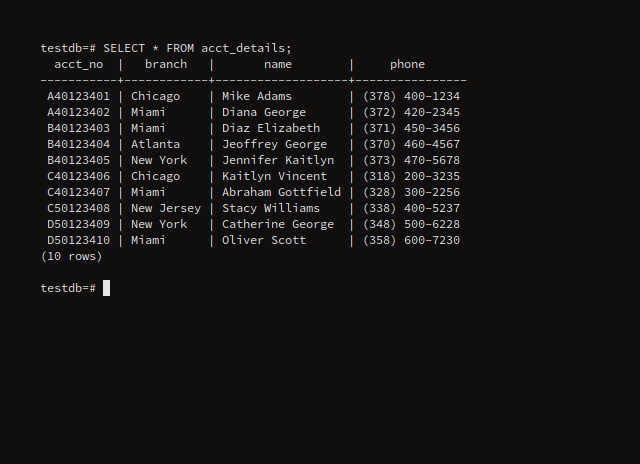
\includegraphics[width=\linewidth]{../Images/Strings/1.png}

\begin{enumerate}
	\item Find the names of all people starting on the alphabet 'D'.\newline
	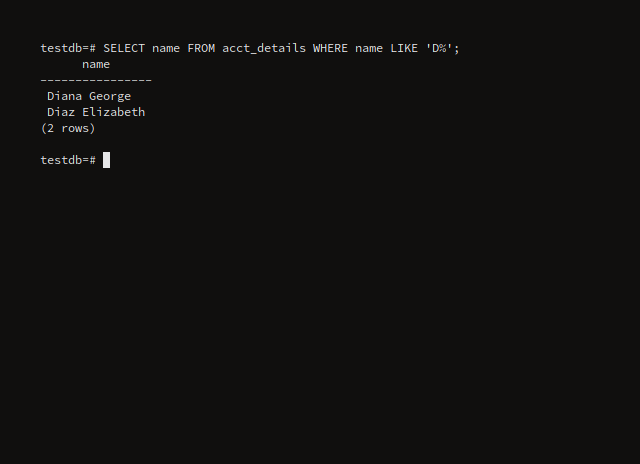
\includegraphics[width=\linewidth]{../Images/Strings/2.png}
	\item List the names of all branches containing the substring 'New'.\newline
	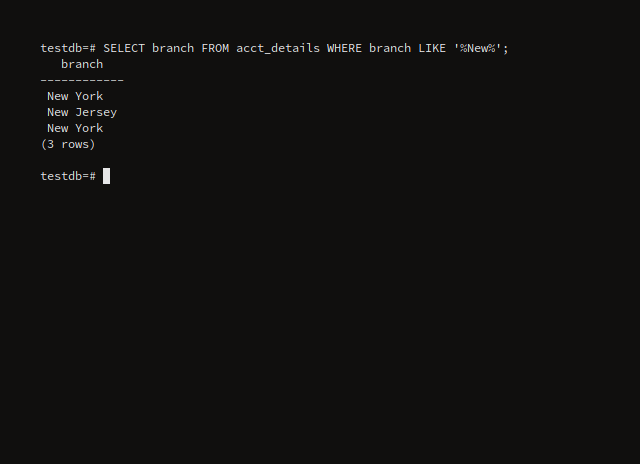
\includegraphics[width=\linewidth]{../Images/Strings/3.png}
	\item List all the names in Upper Case Format.\newline
	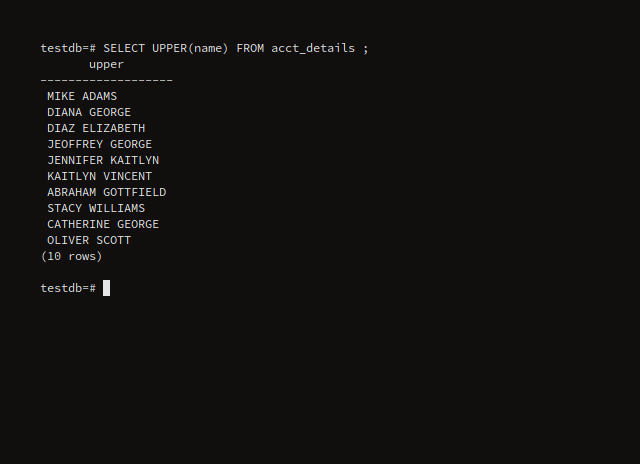
\includegraphics[width=\linewidth]{../Images/Strings/4.png}
	\item List the names where the 4th letter is 'n' and last letter is 'n'.\newline
	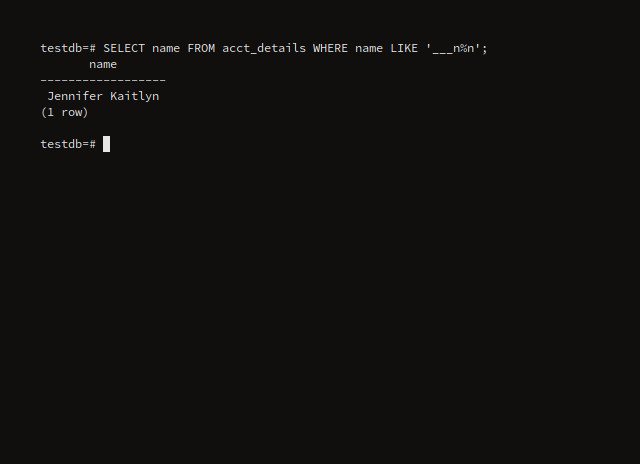
\includegraphics[width=\linewidth]{../Images/Strings/5.png}
	\item List the names starting on 'D' , 3rd letter is 'a' and contains the substring 'Eli'.\newline
	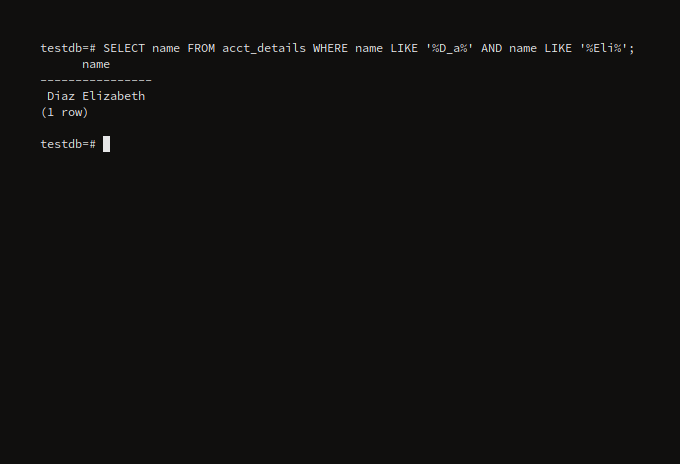
\includegraphics[width=\linewidth]{../Images/Strings/6.png}
	\item List the names of people whose account number ends in '6'.\newline
	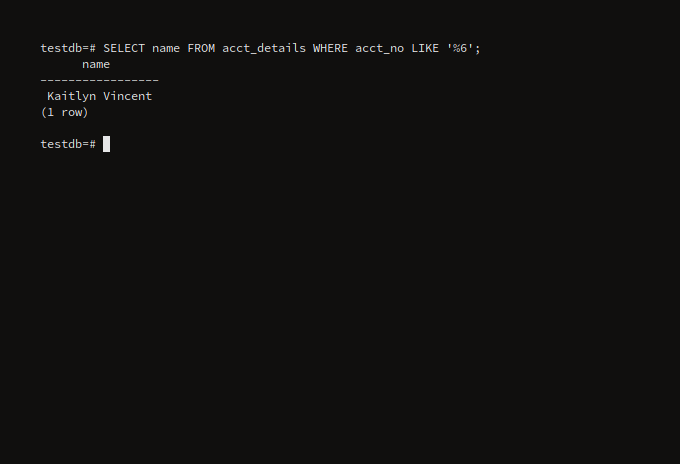
\includegraphics[width=\linewidth]{../Images/Strings/7.png}
	\item Update the table so that all the names are in Upper Case Format.\newline
	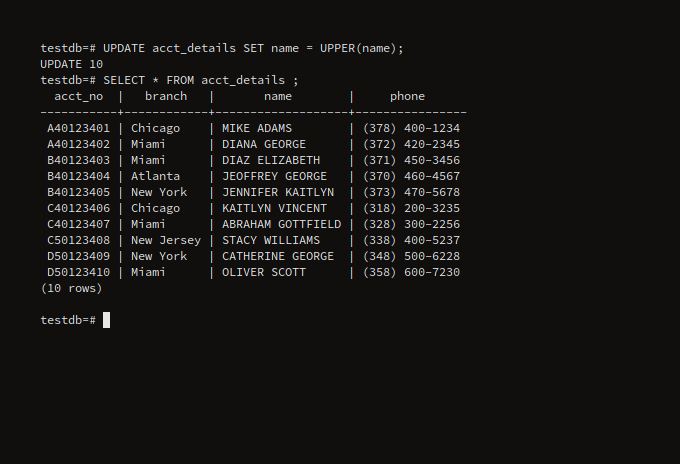
\includegraphics[width=\linewidth]{../Images/Strings/8.png}
	\item List the names of all people ending on the alphabet 't'.\newline
	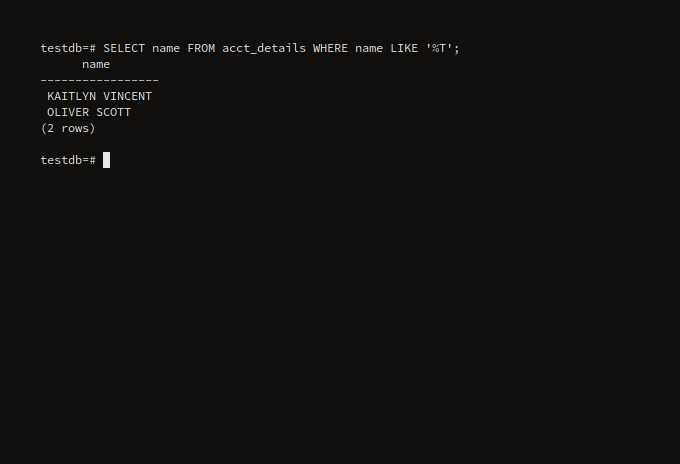
\includegraphics[width=\linewidth]{../Images/Strings/9.png}
	\item List all the names in reverse.\newline
	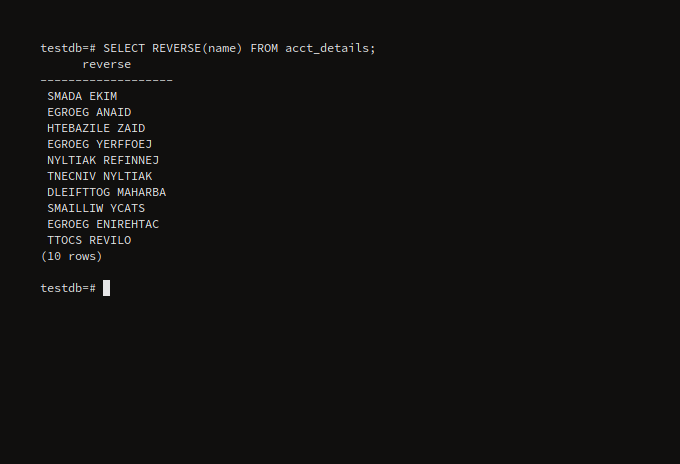
\includegraphics[width=\linewidth]{../Images/Strings/10.png}
	\item Display all the phone numbers including US Country code ( +1). For eg: (378)400-1234 should be displayed as +1(378)400-1234. Use LPAD function.\newline
	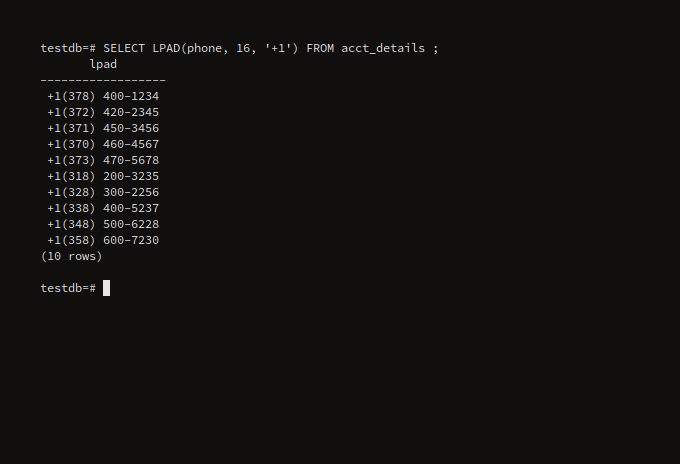
\includegraphics[width=\linewidth]{../Images/Strings/11.png}
	\item Display all the account numbers. The starting alphabet associated with the Account\_No should be removed. Use LTRIM function.\newline
	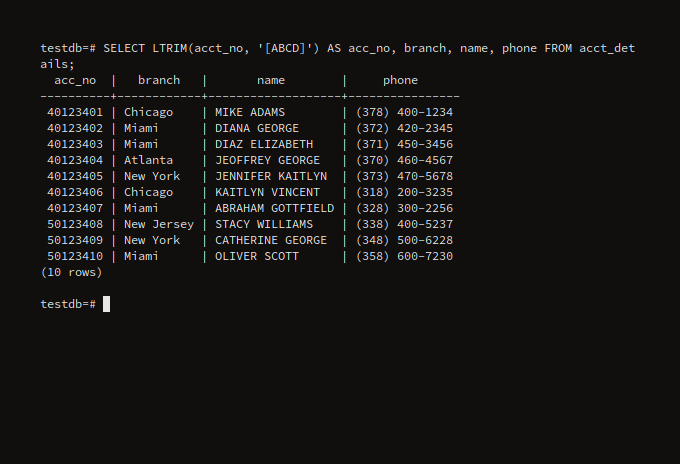
\includegraphics[width=\linewidth]{../Images/Strings/12.png}
	\item Display the details of all people whose account number starts in '4' and name contains the substring 'Williams'.\newline
	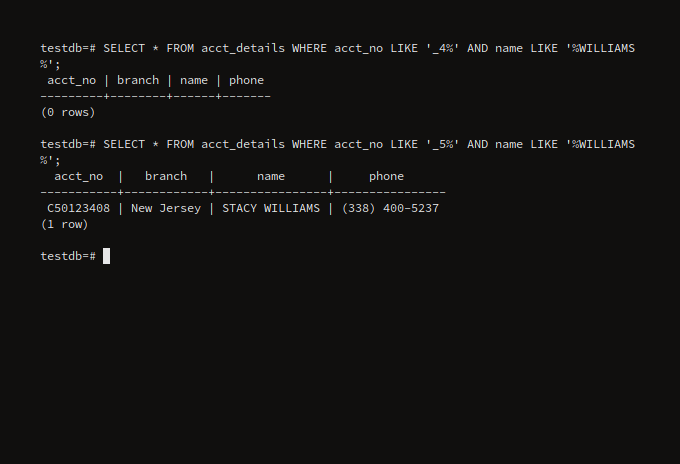
\includegraphics[width=\linewidth]{../Images/Strings/13.png}
\end{enumerate}

\subsubsection{Use the system table DUAL for the following questions:}

\begin{enumerate}
	\item Find the reverse of the string 'nmutuAotedOehT'.\newline
	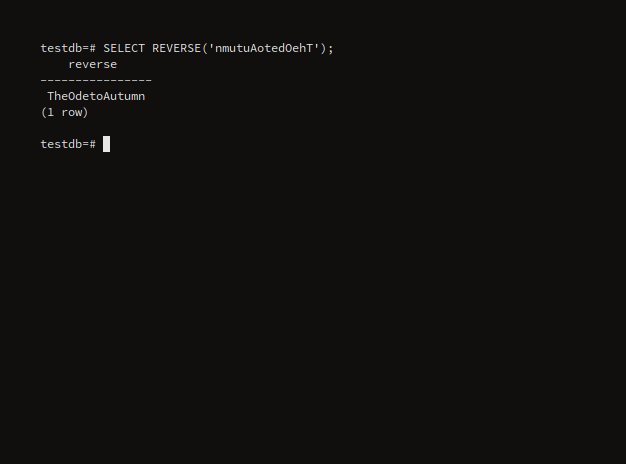
\includegraphics[width=\linewidth]{../Images/Strings/14.png}
	\item Use LTRIM function on '123231xyzTech' so as to obtain the output 'Tech'.\newline
	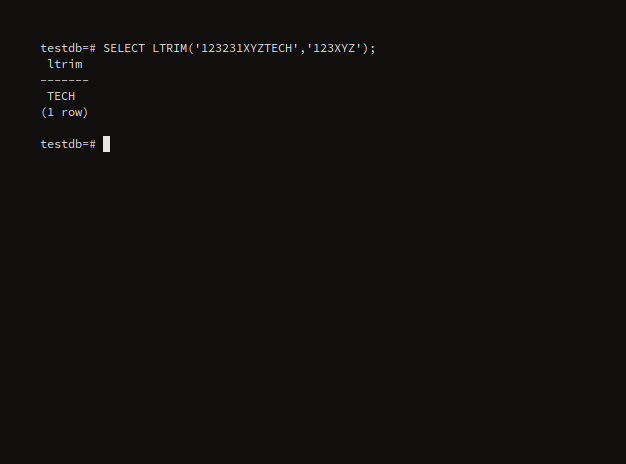
\includegraphics[width=\linewidth]{../Images/Strings/15.png}
	\item Use RTRIM function on 'Computer ' to remove the trailing spaces.\newline
	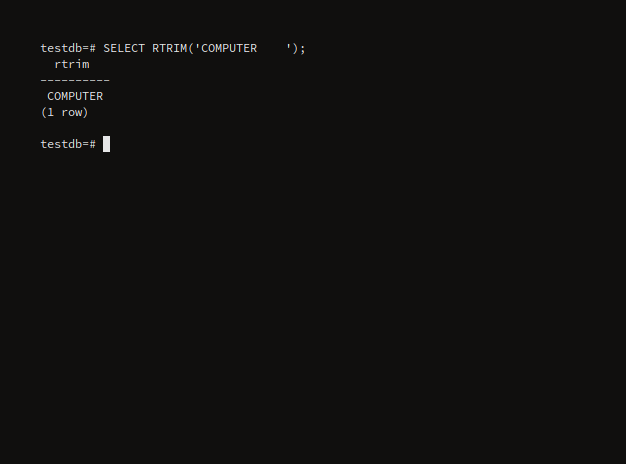
\includegraphics[width=\linewidth]{../Images/Strings/16.png}
	\item Perform RPAD on 'computer' to obtain the output as 'computerXXXX'.\newline
	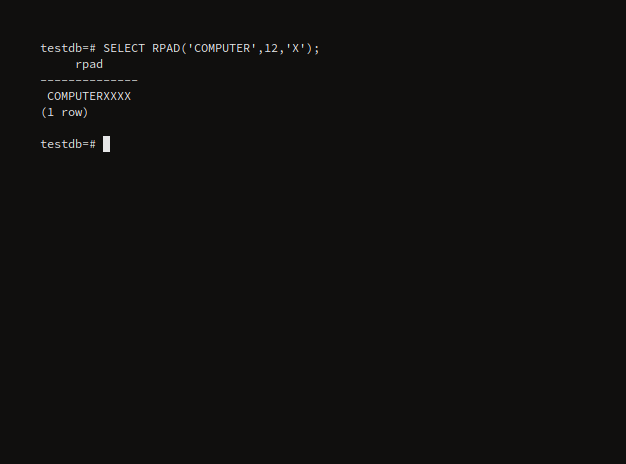
\includegraphics[width=\linewidth]{../Images/Strings/17.png}
	\item Perform INITCAP function on 'mARKcALAwaY'.\newline
	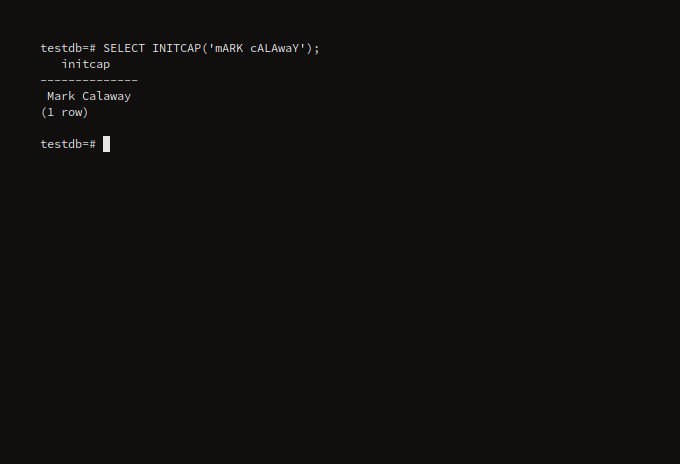
\includegraphics[width=\linewidth]{../Images/Strings/18.png}
	\item Find the length of the string 'Database Management Systems'.\newline
	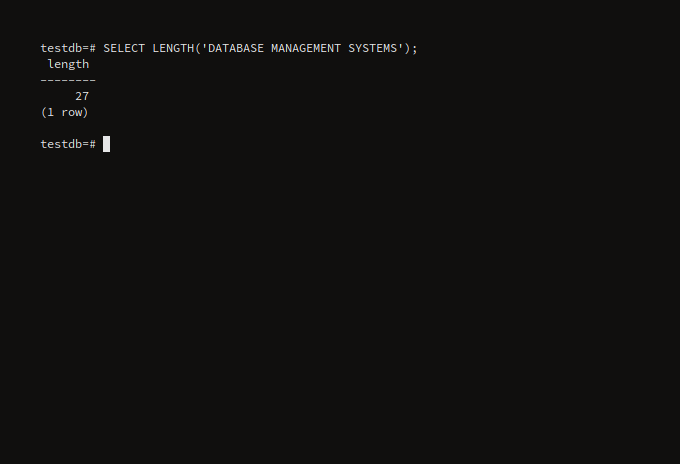
\includegraphics[width=\linewidth]{../Images/Strings/19.png}
	\item Concatenate the strings 'Julius' and 'Caesar'\newline
	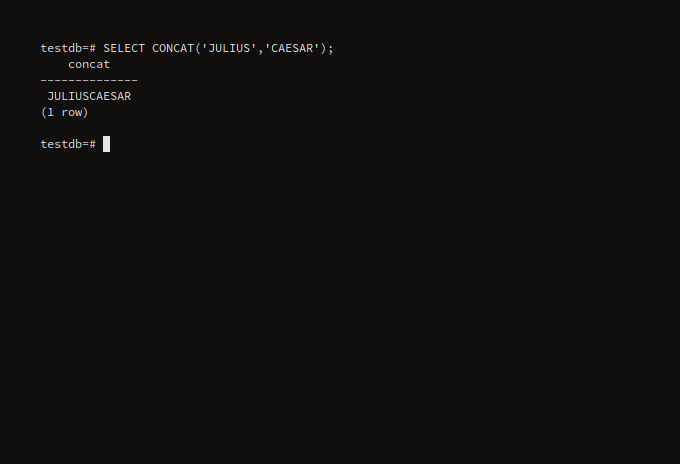
\includegraphics[width=\linewidth]{../Images/Strings/20.png}
	\item Use SUBSTR function to retrieve the substring 'is' from the string 'India is my country'.\newline
	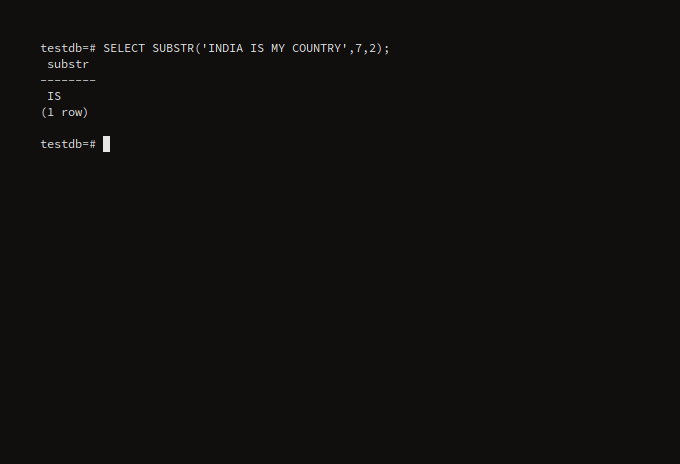
\includegraphics[width=\linewidth]{../Images/Strings/21.png}
\end{enumerate}
}
\end{document}
